\chapter{Receiving Antennas}
Antenna, we recall is a device(transducer) that converts electrical quantities like voltages and currents to electromagnetic waves and also converts electromagnetic waves to electrical quantities. The use of an antenna to convert electromagnetic waves to electrical currents and voltages is discussed in this section of receiving antennas. Under the topic of receiving antennas, we will discuss the characteristics, the power received by the antenna, the response of the antenna to incoming electromagnetic waves in terms of the direction and polarization, and then we will define the relationship between the parameter of the transmitting and receiving antenna.\\

The properties of the transmitting and receiving antenna are related according to the \underline{reciprocity theorem}. This theorem as regards the antenna says that whatever properties an antenna has while it is in transmitting mode, it would have the same properties int he receiving mode. What it essentially means is if an antenna has certain properties for maximum power transfer when in transmitting mode, it would also have these same directions for receiving power maximally in the receiving mode. Also if an antenna has a state of polarization in the transmitting mode, the same antenna in the receiving mode would respond maximally to its state of polarization for an incoming wave.

Consider a simple Hertz dipole shown in fig, \ref{49.1} of length $dl$. Suppose a uniform plane wave is incident at an angle $\theta$ with the z axis. The voltage across the terminals of the dipole, $V_{oc}$ called the open circuit voltage is given as the dot product of the incoming electric field and the length of the dipole, $dl$. It means that if the wave is incident at $\theta = 0\ or\ \pi$ there is no voltage induced but at $\theta = 90\deg\ or\ \frac{\pi}{2}$ there is maximum voltage induced between the terminals. With this we can say the reception pattern for this dipole has a directional dependence of $\sin\theta$ which is exactly the same variation as that of the Hertz dipole in the transmitting mode which was $\sin\theta$. So we have a validation that the radiation characteristics or radiation pattern for the transmitting antenna is identical to the directional dependence of the receiving antenna under consideration. Suppose the electric field of the incoming wave is now perpendicular to the plane of the paper as shown in fig. \ref{49.2}(which is represented by the dot.)
\begin{figure}
	\centering
	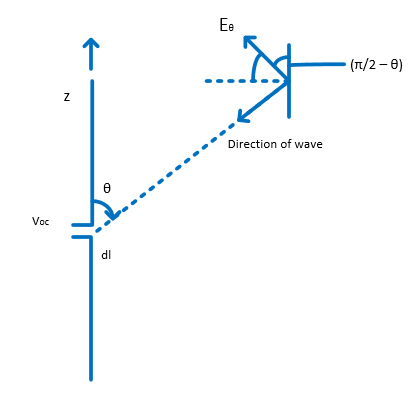
\includegraphics[height=5cm]{fig52__1}
	\caption{}
	\label{49.2}
\end{figure}

The $\vec{E}\cdot d\vec{l}$ which is the induced voltage is zero which means for any orientation of the electric field, it is the component of that electric field which lies in the plane of the paper that induces voltage in the antenna. Thus if we consider a circle of radius $r$ around the dipole antennas, we can say that for any incoming wave, the electric field which is perpendicular to the circle at that point gives zero induced voltage. Therefore the antenna under consideration is responding to only the $\theta$ component of the electric field that is the electric field tangential to the circle and this is precisely the behaviour we have for the Hertz dipole that we have studied. We know that for the Hertz dipole the electric field is linearly polarized and the linear polarization is in the $\theta$ direction. So both the transmitting and receiving antennas have similar polarization characteristics as we would expect from the reciprocity theorem. It is important to know that the reciprocity theorem applies to all antennas in general. The circuit model of the transmitting antenna is shown in fig. \ref{49.3} and it is  known to be the equivalent of an input impedance $Z_{in}$ across terminals.

%\begin{figure}
	%\centering
  %	\includegraphics[width=0.7\linewidth]{fig52.2}
%	\caption{Circuit model of a transmitting antenna}
%	\label{49.3}
%\end{figure}


The input impedance Z$_{in}$  comprises the radiation due to radiation field and  reactive fields (electrostatic and induction fields) generated in the near-region of the antenna .
By reciprocity theorem, the impedance between the terminals of the antenna is identical when the antenna is transmitting and receiving, so if we consider an antenna now operating in the receiving mode which is connected to a load $Z_{l}$ as shown in fig 4, the internal impedance will be the same as $Z_{in}$.

\begin{figure}[h]
	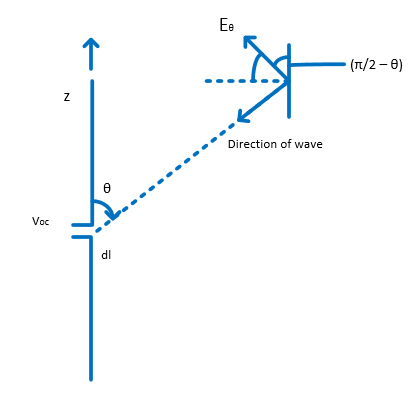
\includegraphics[height=5cm]{fig52__1}
	\centering
	\caption{Hertz dipole as a receiving antenna}
	\label{fig 1}	
\end{figure}


Across the terminals of the antenna there would be an induced voltage, $V_{oc}$ which is due to the incident waves on the antenna. From the circuit in fig 4 we would like to determine the maximum power that is delivered to the load $Z_{l}$,for maximum power transfer, the following conditions would have to be satisfied:

\paragraph*{(a)} The load $Z_{L}$ is a complex conjugate of the internal impedance of the antenna

\paragraph*{(b)} The wave which is incidented on the antenna is coming from the direction of the antenna's maximum response and

\paragraph*{(c)} The polarization of the wave is the same as that of the antenna.\newline

Under these conditions we have maximum power transfered to the load.\\
From fig 4; Current flowing through the circuit, $I=\dfrac{V_{oc}}{2R}$ \\
$Z_{L}=R-JX$; Maximum power delivered $P_{L}=\Re e\left\{VI^{*}\right\}$
\newline Voltage across the load $Z_{L}$, $V={\dfrac{R-jX}{2R}}V_{oc}$ 


$$P_{L}=\Re e\left\{\dfrac{(R-jX)|V_{oc}|^{2}}{4R^{2}}\right\}$$




$$P_{L}=\dfrac{|V_{oc}|^{2}}{4R}$$



This is the maximum power delivered to the load under fully matched conditions and fully matched conditions means we have the direction of maximum radiation and polarization and complex conjugate match.


{if} we consider a wave which is incident on the antenna as shown in fig 4, that has a power density (poynting vector). The antenna due to this incident wave has extracted a power, $P_{L}$ which is the power that is made available to the load. So if we take the ratio of the power $P_{L}$ with the poynting vector (in $Watts/m^{2}$) then the quantity we would get, would have a dimension of area and this quantity is called the effective aperture of the receiving antenna. The parameter is peculiar to receiving antennas only. The effective aperture is denoted by $A_{e}$ and in some cases it is comparable to the physical area of the antenna.
\newline

If S is the power density of the incident wave then,
\newline $A_{e}=\dfrac{P_{L}}{S}$ ,This aperture can be seen as a piece which a receiving antenna has such that for each incoming wave of a certain power density,the antenna effectively cuts some power with this piece which is delivered to the load.
\newline

Essentially we define the effective aperture as a show of the power capturing characteristics of the antenna when a wave impinges on it. Like it was said earlier that the effective aperture in some cases is comparable to the physical area of the antenna, some examples of such cases is the parabolic dish which we will investigate later. Cases where it is not comparable is the thin dipole antenna, the physical area is extremely small but the effective aperture is substantial.
\newline 

Now lets derive a relationship between the unique parameter for receiving antenna and the directivity which also is an important parameter for the transmitting antenna because it shows the focusing capability of antenna. Looking at both parameters, in some sense there is a relationship. Let consider a parabolic dish for instance. If the area of the dish is increased the directivity increases which also means the effective aperture increases because the capturing capabilities is increased. Intuitively, there is a linear relationship so lets derive a general relationship between effective aperture and the directivity of the antenna. We will approach this problem through study of a transmit-receive antenna system and their circuit model. Consider fig 5, the general case of two antennas, the transmitting and receiving antenna separated by some distance r, both of which essentially couple through radiation. Also the equivalent circuit is given

\begin{figure}
	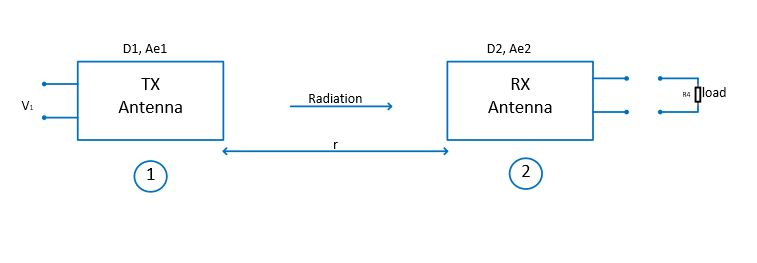
\includegraphics[width=1\linewidth]{fig52__5a}
	\centering
	\caption{Equivalent Circuit}
	\label{fig5b}	
\end{figure}

\begin{figure}
	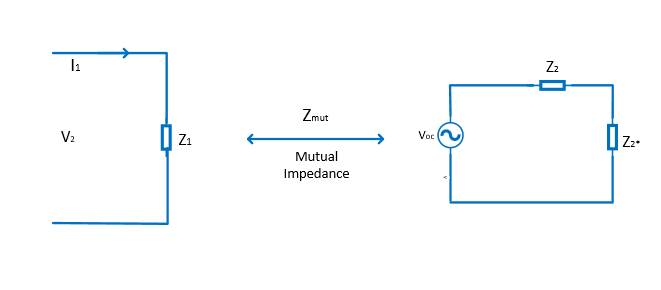
\includegraphics[width=1\linewidth]{fig52_5b}
	\centering
	\caption{Equivalent Circuit}
	\label{fig 1}	
\end{figure}

In fig \ref{fig5b} for the transmit-receive antenna system with a voltage $V_1$, applied to the terminals of the transmitting antenna that supplies current $I_{1}$ to the input impedance $Z_{1}$. The effect of the coupling of the field between these antennas is accounted for by an electrical quantity called the mutual impedance. It depends on the spacing and relative orientation between the antennas, as well as the characteristics of the surrounding medium. It is a parameter that is independent of direction which is a critical property from reciprocity theorem ie independent of which of the antenna is transmitting or receiving $Z_{mut}$ remains the same. For the receiving antenna we have the open circuit voltage $V_{oc}$ across the terminals that supplies the internal impedance, $Z_{2}$ and the load $Z_{2}^*$ (conjugate of $Z_{2}$) for max power transfer.
\newline
The voltage induced across the terminals of the receiving antenna (Antenna 2) is dependent on the current $I_{1}$ is given as

\begin{equation}
\label{49.1}
V_{oc}= I_{1}Z_{mut}
\end{equation}

Then for complex conjugate matched load in antenna (2) the maximum power received for $Z_{2} = R_{2}+jX_{2}$ is given as

$$P_{L}=\dfrac{|V_{oc}|^{2}}{4R_{2}}\
\text{\ substitute\  \ref{49.1}}$$

\begin{equation}
	P_{L} = \dfrac{|I_{1}|^{2}|Z_{mut}|^{2}}{4R_{2}}
\end{equation}


The power transmitted is related to the radiation resistance of antenna 1, so, if $Z_{1}=R_{1}+jX_{1}$,

\begin{equation}
\label{49.3}
\text{Power transmitted}\ P_{t}=|I_{1}|^{2}R_{1}
\end{equation}




As we have discussed, antenna propagates spherical wave in space, so for antenna 1, the wave travels a distance of r and as such has a power density given as $\dfrac{P_{t}}{4\pi r^{2}}$ for an isotropic antenna. However for antenna 1 of directivity $D_{1}$, the power density for a completely matched radiation pattern is given as

$$ S=\dfrac{P_{t} D_{1}}{4\pi r^{2}}\ \text{substitute \ref{49.3}}$$
\begin{equation}
	= \dfrac{|I_{1}|^{2}R_{1}D_{1}}{4\pi r^{2}}
	\label{eqn17b}
\end{equation}
Also power received $P_{l}$ is related to the effective aperture by\\ 
$P_{L}= A_{e_{2}}S$ Substitute \ref{49.3} and equating it to \ref{49.1}\newline
Power received by $R_{\textnormal{x}}$ antenna

$$ P_{L} = A_{e_{2}}\dfrac{|I_{1}|^{2}R_{1}D_{1}}{4\pi r^{2}}$$
$$ = \dfrac{|I_{1}|^{2}R_{1}|Z_{mut}|^{2}}{4R^{2}}$$
Rearranging the expression 
\begin{equation}
\label{49.4}
|Z_{mut}|^{2}=\dfrac{R_{1}R_{2}D_{1}A_{e_{2}}}{\pi r^{2}}
\end{equation}


Now lets interchange the roles of both antennas such that antenna 2 becomes the transmitting antenna and antenna 1 is the receiving antenna . we have said earlier that the $Z_{mut}$ parameter is the same irrespective of which antenna is transmitting or receiving so we can rewrite the expression in equation \ref{49.4} as 

\begin{equation}
\label{49.5}
|Z_{mut}|^{2}=\dfrac{R_{1}R_{2}D_{2}A_{e_{2}}}{\pi r^{2}}
\end{equation}


Equating \ref{49.4} and \ref{49.5} gives $D_{1}A_{e_{2}}= D_{2}A_{e_{1}}$

\begin{equation}
\dfrac{D_{1}}{A_{e_{1}}}= \dfrac{D_{2}}{A_{e_{2}}}
\end{equation}
\newline

This shows that the ratio of the directivity of an antenna to the effective aperture is independent of the pair of antennas we choose, hence it is a constant. The value of the constant can be evaluated by considering the relationship between the directivity and effective aperture of any antenna.

So, lets consider the simplest antenna, the hertz dipole. The radiation pattern for the hertz dipole is $\sin\theta$, when $E=K\sin\theta$, when $K=1$, we have $E_{n}=\sin\theta$

$$\text{Directivity} \ D=\dfrac{4\pi}{\int_{0}^{2\pi}\int_{0}^{\pi}|E_n(\theta , \phi)|^{2} \sin\theta d\theta d\phi}$$

$$ D=\dfrac{4\pi}{\int_{0}^{2\pi}\int_{0}^{\pi}\sin^{2}\theta \sin\theta d\theta d\phi}$$

$$ D=\dfrac{4\pi}{2\pi\int_{0}^{\pi}\sin^{2}\theta \sin\theta d\theta}$$

$$ D=\dfrac{2}{\int_{0}^{\pi}\sin^{2}\theta \sin\theta d\theta} = \dfrac{2}{\int_{0}^{\pi}(1-\cos^{2})\theta \sin\theta d\theta} $$



let $\cos\theta = t$



$\dfrac{dt}{d\theta}=-\sin\theta$
$$ D=\dfrac{2}{-\int_{0}^{\pi}(1-t^{2})dt} = \dfrac{2}{\dfrac{4}{3}} $$


Next we calculate the effective aperture $A_{e}$ of the Hertz dipole; for the Hertz dipole, lets assume a wave is incident on it from the maximum direction $(\theta=\dfrac{\pi}{2})$, and has an electric field $\bar{E}$. So the poynting vector S is given as 
$$ S= \dfrac{1}{2}\dfrac{|E|^{{2}}}{\eta} \ where \  \eta =120\pi$$
$$ S= \dfrac{|E|^{{2}}}{240\pi}$$
\newline

Also let the length of the dipole be dl then the voltage across the terminals
\begin{equation}
V_{oc}=Edl
\label{eqn21}
\end{equation}

The Average Power delivered to the load is given as
\begin{equation}
P_{l}=\dfrac{1}{2}\Re e [VI^{*}]=\dfrac{1}{8}\dfrac{|V_{oc}|^{2}}{R_{ad}}
\label{eqn22}
\end{equation}

from the circuit shown in fig \ref{fig6} where $Z_{int}=R_{rad}+jX_{int} $ for the internal impedance 

\begin{figure}[h]
	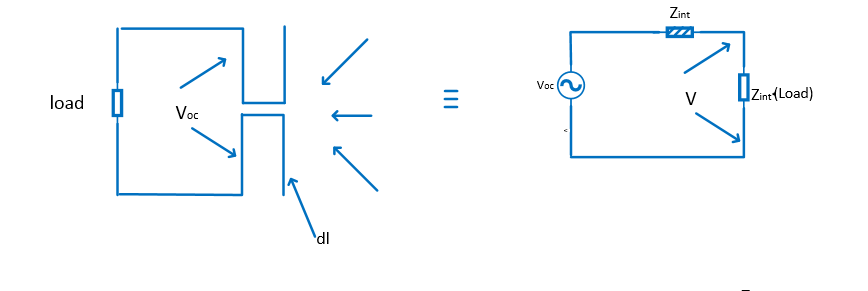
\includegraphics[width=1\linewidth]{fig52_6}
	\centering
	\centering
	\caption{equivalent circuit of a hertz dipole}
	\label{fig6}	
\end{figure}
We recall that the radiation resistance for the Hertz dipole is given as $R_{rad}=80\pi^{2}(\dfrac{dl}{\lambda})^{2}$
\\
substituting $R_{rad}$ and equation \ref{eqn21} in equation \ref{eqn22} gives; 
\\
$$	P_{l}=\dfrac{1}{8}\dfrac{|E|^{2}dl^{2}}{80\pi^{2}}\times\left(\dfrac{\lambda}{dl}\right)^{2}= \dfrac{|E|^{2}\lambda^{2}}{640\pi^{2}}$$


Then the effective aperture $A_{e}=\dfrac{P_{l}}{8}=\dfrac{|E|^{2}\lambda^{2}\times40\pi^{2}}{|E|^{2}\times640\pi^{2}}$

$$=\dfrac{3}{8}\dfrac{\lambda^{2}}{\pi}$$
\newline

Firstly, it is important to note that for the Hertz dipole the effective aperture is independent of length of the dipole and it is an interesting property of the Hertz dipole. Also the Directivity is not a function of length. The second important observation to note is that the effective aperture varies as $\lambda^{2}$ which means as frequency decreases the effective aperture increases.
\paragraph{}Now , lets find the ratio  of the directivity of the Hertz dipole to the effective aperture i.e,
$$\dfrac{D}{A_{e}}=\dfrac{\dfrac{3}{2}}{\dfrac{3}{8}\dfrac{\lambda^{2}}{\pi}}= \dfrac{4\pi}{\lambda^{2}}$$ \ which is the relationship that binds any pair of transmit-receive antennas
\newline

Therefore
\begin{equation}
\label{49.9}
D=\dfrac{4\pi A_{e}}{\lambda^{2}}
\end{equation}

Equation \ref{49.9} relates the effective aperture of an antenna and the directivity of the antenna. So as directivity of the antenna increases the effective aperture also increases. Also, since directivity is related to the beam width of the antenna then the narrower the beam the wider the effective aperture.
\newline

We derived the expression in equation \ref{49.9} for maximum reception for the receiving antenna which is also the case for transmitting antenna corresponding to maximum radiation. However , if the wave is transmitted in any arbitrary direction then we define a new parameter called the directive gain, which is the enhancement or decrease in that direction. The direction in equation \ref{49.9} still holds for any direction and for any antenna.

So, the derivative gain in any direction $(\theta, \varphi)$ 

\begin{equation}
\label{49.10}
G(\theta, \varphi)=\dfrac{4 \pi A_{e}(\theta, \varphi)}{\lambda^{2}}
\end{equation}
\paragraph{} Where $A_{e}(\theta, \varphi)$ is the effective aperture of the antenna for an incoming wave in any arbitrary direction

\begin{figure}[h]
	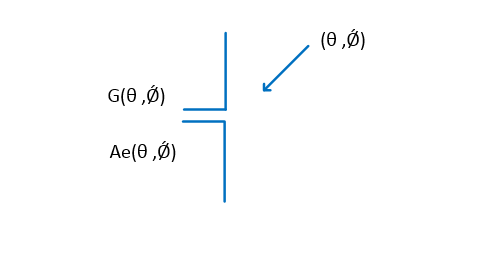
\includegraphics[width=1\linewidth]{fig52_7}
	\centering
	\centering
	\caption{}
	\label{fig 1}	
\end{figure}



However, if we take a direction which gives maximum reception or maximum radiation then equation \ref{49.10} becomes equation \ref{49.9}


Therefore, the maximum value of $G(\theta, \varphi)$ is the directivity D
$$G(\theta, \varphi)max=Directivity$$

\section*{\centering Case Study}
Lets examine a parabolic dish and determine what the effective aperture and directivity is for the antenna. Consider a dish of diameter, $D_{d}$ whose beam width is approximately $\theta\approx \frac{\lambda}{D_{d}}$ in radians (i.e the half power beam width). The beam of the antenna is circular.
\section*{\centering solution}


$$Directivity=\dfrac{4\pi}{\int_{\phi=0}^{2\pi}\int_{\theta=0}^{\pi}|E(\theta,\varphi)|^{2}\sin^{2}\theta \sin\theta d\theta d\varphi} $$
\newline

The denominator of the above equation is the volume of the three dimensional radiation pattern (i.e normalized electric field) which can be seen as a cylinder of height given as 1 unit and diameter given as $\theta$.

So $\int_{\phi}^{2\pi}\int_{\theta}^{\pi}|E(\theta,\phi)|^{2}\sin^{2}\theta \sin\theta d\theta d\phi \approx \pi\left[\dfrac{\theta}{2}\right]^{2}$ this is the solid angle $\Omega$

substitute $\theta = \dfrac{\lambda}{D_{d}}$ gives  $\pi\left[\dfrac{\pi}{2D_{d}}\right]^{2}$

$$So \ Directivity, D= \dfrac{4\pi}{\left[\dfrac{\pi}{2D_{d}}\right]^{2}} = \frac{16D_{d}^{2}}{\lambda^{2}}$$

$$Also \ A_{e}=\frac{\lambda^{2}}{4\pi} \cdot D = \frac{\lambda^{2}}{4\pi} \cdot \frac{16D_{d}^{2}}{\lambda^{2}} = \frac{16}{4\pi}D_{d}^{2} = \frac{4}{\pi}D_{d}^{2}$$

\paragraph{}This tells us that the physical area $\frac{\pi D_d^2}{4}$ of this parabolic dish is comparable to the effective aperture of this antenna.

\paragraph{}In conclusion, the relationship $D=\frac{4\pi A_{e}}{\lambda^{2}}$ is extremely important as one can easily switch from the properties of a transmitting antenna to that of the receiving antenna and vice versa.